\chapterillustration{abertura-semelhanca}{abertura-semelhanca-professor}

\chapterwhat{São estudadas a semelhança de figuras geométricas, os casos de semelhança de triângulos e polígonos, e suas aplicações.}


\chapterbecause{Em primeiro lugar, o conceito de semelhança está presente em diversos contextos e sua compreensão permite compreender melhor o mundo que vivemos. Por outro lado, a semelhança de triângulos é um instrumento importante para obter propriedades métricas e relações entre elementos de polígonos. Por fim, a semelhança de triângulos é uma ferramenta muito útil na resolução de problemas de geometria, tanto plana quanto no espaço.}

\chapter{Semelhança}


%%%% Página de créditos

% Autores
\autorum{Eduardo Wagner}
\autordois{Marcos Paulo}

% Revisores
\revisorum{Cydara Ripoll}
\revisordois{Letícia Rangel}

\autordacapa{Pradeep Gopal}{Unsplash}{https://unsplash.com/photos/6uJDEQx-cho}
\versao{1.0}

\ilustracao{Miller  Guglielmo}

\graficos{Beatriz Cabral}

\ccbysa
 
\creditos

\mainmatter

\begin{apresentacao}{Introdução}
A Matemática elementar caminha apoiada em dois pilares: os números e as formas. Neste capítulo de Semelhança reunimos a proporcionalidade (números) com as figuras geométricas (formas). Os alunos possuem internalizado o conceito de Semelhança desde o final do Ensino Fundamental, quando praticaram atividades de ampliar figuras dadas em um reticulado, mas além disso, sempre tiveram contato com miniaturas ou outros brinquedos representando modelos reduzidos de objetos reais.

Como indica a \href{http://historiadabncc.mec.gov.br/documentos/bncc-2versao.revista.pdf}{Base Nacional Comum Curricular}  (BNCC) para o primeiro ano do Ensino Médio, a Semelhança servirá de base para o desenvolvimento de dois temas imediatos:
\begin{enumerate}
\item {} 
O teorema de Pitágoras e suas aplicações na geometria plana e na geometria espacial e,

\item {} 
as razões trigonométricas tanto no triângulo retângulo quanto em triângulos quaisquer e suas diversas aplicações.

\end{enumerate}

Esses dois objetivos estão bem claro nas duas habilidades da BNCC e mostramos a seguir.

\begin{habilities}{EM12MT02}

Resolver e elaborar problemas utilizando a semelhança de triângulos e o teorema de Pitágoras, incluindo aqueles que envolvem o cálculo das medidas de diagonais de prismas, de altura de pirâmides, e aplicar esse conhecimento em situações relacionadas ao mundo do trabalho

\tcbsubtitle{EM12MT03}

Utilizar a noção de semelhança para compreender as razões trigonométricas no triângulo retângulo, suas relações em triângulos quaisquer e aplicá-las em situações como o cálculo de medidas inacessíveis, entre outras
\end{habilities}

Deve-se destacar que para a exploração e o desenvolvimento das habilidades acima será necessário compreender e saber utilizar, apenas, a semelhança de triângulos. Entretanto, o capítulo apresenta uma definição geral de semelhança por duas importantes razões. Em primeiro lugar porque o estudante reconhece, desde muito jovem, a ampliação ou redução de imagens diversas (retratos, por exemplo) e este é o momento adequado para mostrar a parte da matemática que explica essa transformação. Em segundo lugar, porque o conceito geral será necessário em outros momentos da sua aprendizagem. No momento de estudar, por exemplo, a área do círculo, o professor diz (ou o livro diz) que duas circunferências quaisquer são semelhantes. O aluno sente que isso é verdade, mas não consegue explicar se não conhece a definição geral de semelhança. Por outro lado, na geometria do espaço o livro vai dizer que se cortarmos um cone por um plano paralelo à sua base, obteremos um cone menor semelhante ao primeiro. E o que significa que um cone seja semelhante a outro? Assim, percebemos que não é suficiente que o aluno conheça apenas a semelhança de triângulos. É necessário, portanto, que ele conheça o que realmente é uma Semelhança.

O capítulo se inicia com uma atividade que recorda o que o aluno fez na escola quando muito mais jovem: a ampliação de um desenho sobre um fundo quadriculado. Mesmo sendo uma atividade algo infantil, o conceito de semelhança aparece e uma interessante questão é abordada: qual é a diferença entre “semelhante” e “parecido”. Na linguagem comum, usamos essas palavras praticamente da mesma forma, mas na Matemática, a primeira tem definição precisa e a outra não.

A seção Explorando mostra exemplos de figuras semelhantes e recomenda que os alunos vejam um interessante desenho da Disney que aborda diversos aspectos da Matemática na vida diária, inclusive a Semelhança.

Em seguida, aparece a Atividade Plantas Baixas, que é uma atividade motivadora. Nessa atividade não há o objetivo que o aluno consiga responder a todas as perguntas, mas sim que o aluno se sinta provocado a aprender o material do capítulo para poder respondê-las. Essa atividade será retomada adiante quando o aluno terá então as ferramentas necessárias para responder as questões com toda segurança.

No Organizando as Ideias aparece de início a definição geral de Semelhança com vários exemplos mostrando o que é a razão de semelhança entre duas figuras e o que significa o fator de ampliação de uma figura para outra. A importância da semelhança de triângulos é enfatizada e as atividades seguintes procuram fazer com que o aluno compreenda bem o conceito de Semelhança o teorema central da semelhança de triângulos.

A Atividade Teorema Central da Semelhança de Triângulos tem grande importância pois nela se pede ao aluno que leia um texto contendo a demonstração de um teorema. Precisamos lembrar que, até esse ponto do aprendizado, o professor (em geral) teve o costume de explicar aos alunos toda a matéria e os alunos, é claro, se acostumaram com esse procedimento. Agora, pela primeira vez, se solicita ao aluno que leia um pequeno texto, compreenda e aprenda sozinho, o que representa um grande salto no processo de aprendizagem. Entendemos que uma das coisas mais importantes que o professor pode ensinar a seus alunos é ensiná-los a aprender sozinhos.

As atividades seguintes conduzem o aluno a aplicar seus conhecimentos em situações bem diferentes, incluindo aquelas em que ele terá que interferir na figura para criar os triângulos semelhantes que vão possibilitar a resolver determinada questão.

O capítulo termina com os Exercícios, alguns de manipulação apenas dos triângulos semelhantes, mas outros bem contextualizados, incluindo um de cálculo de distância inacessível, contemplando o que solicita a \textbf{EM12MT02}.
\end{apresentacao}

\explore{Figuras Semelhantes}


Quando nos afastamos de uma figura, ou quando damos um zoom em uma foto com a câmera do celular, a forma e as proporções são mantidas e apenas o seu tamanho muda. É disso que vamos falar no início deste capítulo de Semelhança. Além do conceito de semelhança que permite entender bem o que seja ampliar ou reduzir uma imagem, a semelhança de triângulos também se mostrará uma ferramenta muito poderosa para resolver muitos problemas de geometria.


Você consegue reproduzir a imagem abaixo dentro de um quadrado com $5$ cm de lado?

\begin{texto}
{
\begin{observation}
Para ampliar uma figura, um método prático é o de sobrepor à figura uma malha regular. Ampliando a malha os pontos de referência da figura sobre a malha inicial poderão ser transferidos sem dificuldade para a nova malha ampliada e assim, todos os delalhes da figura inicial poderão aparecer na nova figura em tamanho maior.
\end{observation}
}
\end{texto}

\begin{figure}[H]
\centering

\noindent\includegraphics[width=200bp]{{malha}.png}
\end{figure}



Em princípio, para ampliar uma figura, qualquer malha regular serve. Entretanto, a malha mais simples é a quadriculada, que já é familiar aos alunos desde o ensino fundamental e, por essa razão, o Cebolinha já está com a malha quadriculada proposta, faltando ao aluno, apenas completar as linhas sobre o desenho para poder transportar os pontos importantes da figura para a nova malha ampliada.
Essa atividade inicial é, naturalmente, opcional. Há alunos que gostariam de fazer essa experiência e, certamente, outros que possam considerar infantil tal proposta. Entretanto, o objetivo que é o de introduzir a noção de ampliação terá sido realizado.

A figura que você pretende criar deverá ser \textit{semelhante} à que está acima, mas se a sua habilidade não for muito boa, ela será apenas \textit{parecida} com a original.

Na linguagem comum usamos essas duas palavras com o mesmo significado, mas em matemática não. A palavra semelhante tem significado preciso e é isso o que veremos neste capítulo.

A semelhança é um conceito que está presente em inúmeras situações da nossa vida. Este conceito está diretamente ligado à percepção de figuras que são essencialmente a mesma, mas apresentadas em tamanhos e posições diferentes. Essa é a essência do conceito: a manutenção da forma com apresentação do objeto em tamanhos diferentes.

Não há nenhuma diferença na abordagem da semelhança no mundo 2D (plano) ou no mundo 3D (espacial); tudo funciona exatamente da mesma maneira. Entretanto, neste capítulo, vamos desenvolver a semelhança em figuras planas.

A semelhança é um conceito muito interessante e bastante intuitivo, pois está ligado às ideias de ampliar ou reduzir alguma coisa, ou alguma imagem. Por exemplo, a seguir, você vê três figuras semelhantes.

\clearpage
\begin{sugestions}{Donald no País da Matemágica}
{
O vídeo tem 27 min e aborda diversos aspectos interessantes da Matemática elementar. Há muita coisa para comentar com os alunos, mas você pode selecionar apenas o que se relaciona com a semelhança. Como os alunos ficarão curiosos, em algum momento o vídeo inteiro poderá ser comentado.
}{1}{2}
\end{sugestions}
\begin{objectives}{Plantas Baixas}
{
\begin{itemize}
\item {} 
Reconhecer ampliação ou redução de um objeto.

\item {} 
Estimar a relação entre as medidas de duas figuras semelhantes.

\end{itemize}
}{1}{2}
\end{objectives}
\begin{sugestions}{Plantas Baixas}
{
Esta atividade visa principalmente despertar o aluno para as informações que ele pode obter a partir do conceito que será abordado no capítulo. É fundamental que o aluno possa experimentar sua intuição a respeito do tema.

\begin{itemize}
\item {} 
A ideia de que a planta de uma casa mostra um desenho reduzido da situação real deve ser abordada de forma a explorar a intuição dos alunos. Inicialmente, não diga nada, não explique nada; deixe que eles descubram sozinhos o conceito de escala de um desenho.

\item {} 
Depois que os alunos estiverem na direção certa, você deve explicar o conceito de proporcionalidade.

\item {} 
A regra de três é a ferrramenta da proporcionalidade. Conhecendo três termos de uma proporção podemos calcular o quarto.

\item {} 
A atividade a seguir, vai mostrar a necessidade de termos ferramentas adequadas para calcular certas distâncias.

\end{itemize}
}{1}{2}
\end{sugestions}
\clearmargin
\begin{answer}{Plantas Baixas}
{
\begin{enumerate}
\item {} 
Espera-se apenas que o aluno diga que não é possível calcular a área do quarto 2, mas há sempre a possibilidade do aluno tentar aproximar a forma pentagonal do quarto a um retângulo e isso pode levá-lo futuramente a problemas mais sérios. Fique atento.

\item {} 
Aqui é uma boa oportunidade para falar em escala, proporcionalidade e regra de 3. A resposta esperada é $6{,}75$ m

\item {} 
A resposta esperada é $1{,}72$ m

\end{enumerate}

Como essa atividade é introdutória ao capítulo não há respostas precisas. Para qualquer item, uma resposta  “não sei”  é expressiva. Ela mostrará que o aluno que deu essa resposta não traz do ensino fundamental algum conhecimento relacionado com essa situação, e isso é importante. Entretanto, outros poderão, mesmo sem conhecer a proporcionalidade, estimar as medidas usando apenas a intuição. Isso também é importante e uma avaliação visual será boa se no item \titem{b)} o aluno responder  “um pouco menos que $7$ m”   e no item \titem{c)} responder  “um pouco menos que $2$ m”.
}{1}
\end{answer}
\begin{figure}[H]
\centering
\capstart

\noindent\includegraphics[width=.9\linewidth]{{figuras_semelhantes}.png}
\caption{Skatista}
\label{skatista}
\end{figure}

As figuras semelhantes mostram a mesma “forma”, mas nada diz quanto ao tamanho, ou mesmo com a disposição ou arrumação relativa das figuras. Isso faz com que, apesar do conceito ser intuitivo, a definição não seja muito fácil pois deverá ser precisa.

Para explorar mais, recomendamos um filme muito antigo. Ele se chama \textit{Donald no país da Matemágica} e mostra diversas situações em que a Matemática está presente sem que se perceba. Você vai ver, inclusive, qual é o retângulo mais bonito de todos e o que isso tem a ver com o tema do nosso capítulo: Semelhança.

Veja o filme \href{https://www.youtube.com/watch?v=wbftu093Yqk}{Donald no  País da Matemágica}

\begin{task}{Plantas baixas}

A figura a seguir mostra a planta de uma casa e as medidas indicadas no desenho mostram as dimensões reais em metros. Entretanto, Fabio, uma pessoa que gostaria de ter mais informações sobre essa casa, mediu com sua régua a largura da parede do fundo da casa e, desprezando a espessura das paredes, encontrou $8$ cm, colocando essa informação no desenho.

As perguntas a seguir são importantes para o curioso Fabio. Se você não souber responder, não se preocupe, pois elas estão nessa atividade para que você perceba o que vamos desenvolver neste capítulo. Essa casa será retomada adiante.

\begin{figure}[H]
\centering

\noindent\includegraphics[width=250bp]{{planta_1}.png}
\end{figure}

\begin{enumerate}
\item {} 
O desenho fornece informações suficientes para que se calcule a área do Quarto 2?

\item {} 
Com a régua Fabio mediu a distância entre a porta de entrada e a porta da cozinha e encontrou $9$ cm. Na realidade qual é essa distância?

\item {} 
Fabio mediu também o comprimento da mesa da sala de jantar e encontrou $2{,}3$ cm, Na realidade qual é essa medida?

\end{enumerate}
\end{task}



\needspace{.4\textheight}
\arrange{Figuras Semelhantes}

\paragraph{O que é semelhança para a Matemática?}

Na atividade anterior percebemos que a planta de uma casa é um modelo reduzido da situação real e isso significa que as proporções entre as medidas são mantidas. Dizemos então que a planta da casa e o piso da casa são semelhantes.
Para tornar o conceito preciso precisamos de uma definição.
\begin{observationtitle}{Figuras semelhantes}
Duas figuras \(F\) e \(F'\) são semelhantes quando existe uma correspondência biunívoca entre os pontos de uma e os pontos de outra, de forma que, para quaisquer pontos \(X\) e \(Y\) da figura \(F\) e seus correspondentes \(X'\) e \(Y'\) da figura \(F'\) tem-se que a razão \(\dfrac{XY}{X'Y'}\)   é constante.
\end{observationtitle}

\begin{wrapfigure}[11]{r}{.4\linewidth}

\resizebox{\linewidth}{!}
{
\begin{tikzpicture}
\draw [rotate around={0.:(4.5,4.)},line width=3.6pt,color=\currentcolor!80] (4.5,4.) ellipse (1.8251407699364404cm and 1.0397782600555694cm);]
\draw [rotate around={-45.:(8.629881130634992,5.065307896443685)},line width=3.6pt,color=\currentcolor!80] (8.629881130634992,5.065307896443685) ellipse (2.4274372240154656cm and 1.3829050858739074cm);
\draw [line width=2.pt] (3.96,4.28)-- (5.16,3.6);
\draw [line width=2.pt] (8.385363605700684,5.836478552005733)-- (8.874398655569301,4.068428756326888);
\draw (7.98,7.88) node[anchor=north west] {$F^\prime$};
\draw (5.,4.2) node[anchor=north west] {$Y$};
\draw (3.28,4.58) node[anchor=north west] {$X$};
\draw (8.3,6.5) node[anchor=north west] {$X^\prime$};
\draw (9.0,4.68) node[anchor=north west] {$Y^\prime$};
\draw (2.44,5.24) node[anchor=north west] {$F$};
\draw [fill=black] (3.96,4.28) circle (2.5pt);
\draw [fill=black] (5.16,3.6) circle (2.5pt);
\draw [fill=black] (8.385363605700684,5.836478552005733) circle (2.5pt);
\draw [fill=black] (8.874398655569301,4.068428756326888) circle (2.5pt);
\end{tikzpicture}
}
\caption{Figuras Semelhantes}
\end{wrapfigure}
Vamos entender bem essa definição. Não se impressione se ela lhe parece difícil.

Uma correspondência biunívoca (ou uma bijeção) entre \(F\) e \(F^\prime\) é uma função onde  cada ponto de \(F\) tem um correspondente em \(F'\) e, reciprocamente, cada elemento de \(F'\) tem seu correspondente em \(F\).

Volte para a \Fref{skatista} e veja novamente as duas primeiras representações da skatista. Escolha um ponto da primeira figura, uma ponta do skate, por exemplo. Certamente você saberá encontrar esse mesmo ponto na segunda figura. Por outro lado, se você assinalar qualquer outro ponto da segunda figura, você também saberá localizar onde está o ponto correspondente na primeira figura. Uma vez que você assinalou dois pontos de uma das figuras e seus correspondentes na segunda figura, você pode determinar as distâncias entre esses pares de pontos. A função que relaciona os pontos das duas figuras chama-se uma semelhança se a razão entre essas distâncias for sempre a mesma, \textit{quaisquer que sejam os pontos escolhidos}.

\begin{observationtitle}{Razão de semelhança e fator de ampliação/redução}
Em uma semelhança entre \(F\) e \(F'\), se temos \(\dfrac{XY}{X'Y'}=k\), dizemos que a \textit{razão de semelhança} de \(F\) para \(F'\) é \(k\).

Naturalmente que \(\dfrac{X'Y'}{XY}=\dfrac{1}{k}\)  e assim dizemos que a \textit{razão de semelhança} de \(F'\) para \(F\) é \(\dfrac{1}{k}\).

Fazendo agora \(\alpha=\dfrac{1}{k}\) temos que \(X’Y’=\alpha\cdot XY\)  e dizemos que \(\alpha\)  é o \textit{fator de ampliação} de \(F\) para \(F'\).
\end{observationtitle}

\begin{example}{pequeno e peixe grande}

Na figura a seguir, o fator de ampliação é $2{,}5$. Isso significa que todas as distâncias entre pontos do peixe menor aparecem no peixe maior, multiplicadas por $2{,}5$.

\begin{figure}[H]
\centering

\noindent\includegraphics[width=.75\linewidth]{{peixe}.png}
\end{figure}

Observe que, se no peixe menor alguma distância entre dois pontos mede 2 unidades, então a distância entre os pontos correspondentes no peixe maior será de \(2,5\times 2 = 5\) unidades. Assim, a razão de semelhança do peixe menor para o maior será \(\dfrac{2}{5}\), enquanto que a razão de semelhança do peixe maior para o menor será \(\dfrac{5}{2}\).
\end{example}

\begin{sugestions}{Você Sabia?}
{Os alunos devem observar que existe aqui uma correspondência biunívoca entre as duas figuras. Para cada ponto assinalado em uma delas é possível encontrar o ponto correspondente na outra. Entretanto essas figuras não são semelhantes porque as razões entre distâncias não são as mesmas para todos os pares de pontos}
{1}{1}
\end{sugestions}

\begin{knowledge}

\paragraph{Comprove você mesmo}

Não podemos negar que as figuras abaixo são parecidas, mas devemos reconhecer que não são semelhantes pois as proporções não são todas mantidas.

\begin{figure}[H]
\centering

\noindent\includegraphics[width=.575\linewidth]{{nao-semelhantes_1}.png}
\end{figure}



Hoje em dia, os softwares que fazem reconhecimento de faces, utilizam uma definição matemática para a palavra  “parecido”. É por isso que, em fotos do Facebook, o software permite reconhecer pessoas já identificadas em fotos anteriores. Porém nada disso seria possível sem o primeiro passo, que é a semelhança.
\end{knowledge}
\cleardoublepage

\def\currentcolor{session1}
\begin{objectives}{Triângulos Semelhantes}
{\begin{itemize}
\item {} 
Utilizar a definição de semelhança no lugar da intuição;

\item {} 
Concluir que, no caso de semelhança de triângulos, a definição é equivalente ao caso $LLL$ de semelhança de triângulos

\end{itemize}}
{1}{1}
\end{objectives}
\begin{sugestions}{Triângulos Semelhantes}
{A atividade a seguir, pede que os alunos verifiquem se os triângulos são ou não semelhantes. Em princípio, os alunos podem ficar confusos tentando mostrar que todos os pontos no interior da região triângular atendem o que foi pedido na definição de semelhança. Vale lembrar que um triângulo fica definido por três pontos não colineares e, portanto, basta verificar que as razões entre distâncias \(AB\), \(BC\) e \(AC\) e \(A'B'\), \(B'C'\) e \(A'C'\), respectivamente, são iguais. Desse modo, a figura formada pelos pontos \(A\), \(B\) e \(C\) é semelhante à figura formada pelos pontos \(A'\), \(B'\) e \(C'\).

Portanto, atender à definião de semelhança, no caso de triângulos, consiste no caso de semelhança \(LLL\). Um caso de semelhança de triângulos é um conjunto de condições mínimas que garantem a semelhança dos triângulos envolvidos. Apenas os triângulos possuem casos de semelhança simples o sufuciente para serem estudados e conhecidos.}
{1}{1}
\end{sugestions}
\begin{answer}{Triângulos Semelhantes}
{\begin{enumerate}[topsep=0pt]
\item {} 
Nomeação do professor: \(A\), \(B\) e \(C\) opostos, respectivamente aos lados de comprimentos $6$, $7{,}2$ e $8$ e para $\mathcal\{T\}_1{}$ usaremos as letras \(P\), \(Q\) e \(R\), respectivamente opostos aos lados de comprimentos $9$, $10{,}8$ e $12$.

\item {} 
\((A, P)\), \((B, Q)\) e \((C, R)\)

\item {} 
\((AB, PQ)\), \((BC, QR)\) e \((AC, PR)\)

\item {} 
Calculando as razões:
\begin{itemize}[topsep=0pt]
\item {} 
\(\dfrac{6}{9}=\dfrac{2}{3}\)

\item {} 
\(\dfrac{8}{12}=\dfrac{2}{3}\)

\item {} 
\(\dfrac{7{,}2}{10,{,}8}=\dfrac{2}{3}\)

\end{itemize}

\end{enumerate}

A razão \(\dfrac{3}{2}\) também é uma resposta aceitável. Note que \(\frac{6}{9}=\frac{8}{12}=\frac{7,2}{10,8}=\frac{2}{3}\) e os triângulos são semelhantes na razão \(\frac{2}{3}\) pelo caso \(LLL\)  de semelhança de triângulos.}
{0}
\end{answer}
\explore{Triângulos Semelhantes}



A semelhança de triângulos é uma ferramenta poderosa para resolver inúmeros problemas de geometria. Isso ocorre porque o triângulo tem uma situação especial no que estamos estudando: ao contrário dos outros polígonos, é muito fácil reconhecer quando dois triângulos são semelhantes.

De fato, para triângulos, podemos definir conjuntos de condições mínimas para que possamos afirmar que dois triângulos são semelhantes. Esses conjuntos de condições mínimas são chamados \textit{casos de semelhança de triângulos}.

A própria definição de semelhança entre duas figuras, no caso dessas figuras serem triângulos, resume-se a verificar a proporcionalidade entre seus lados correspondentes. Este é o chamado caso “caso LLL” (lado-lado-lado) de semelhança de triângulos.

\begin{task}{Triângulos semelhantes}

A figura a seguir mostra dois triângulos \(\mathcal{T}_1\) e \(\mathcal{T}_2\).
\begin{center}\begin{tikzpicture}
\begin{scope}[scale=.5]
\fill[line width=1.2pt,color=\currentcolor!80,fill=\currentcolor!80,fill opacity=0.20000000298023224] (-2.4026846239814494,9.01432812261539) -- (-3.1006389948749313,3.0550614146931245) -- (4.239720652539582,6.236117881750678) -- cycle;
\fill[line width=1.2pt,color=cor1,fill=cor1,fill opacity=0.20000000298023224] (7.032280832257959,12.718092698860787) -- (12.293364416514931,1.9328713511339897) -- (17.311287593236727,9.404179602873993) -- cycle;
\draw [line width=0.8pt] (-3.1006389948749313,3.0550614146931245)-- (4.239720652539582,6.236117881750678);
\draw [line width=1.2pt,color=\currentcolor!80] (-2.4026846239814494,9.01432812261539)-- (-3.1006389948749313,3.0550614146931245);
\draw [line width=1.2pt,color=\currentcolor!80] (-3.1006389948749313,3.0550614146931245)-- (4.239720652539582,6.236117881750678);
\draw [line width=1.2pt,color=\currentcolor!80] (4.239720652539582,6.236117881750678)-- (-2.4026846239814494,9.01432812261539);
\draw [line width=1.2pt,color=cor1] (7.032280832257959,12.718092698860787)-- (12.293364416514931,1.9328713511339897);
\draw [line width=1.2pt,color=cor1] (12.293364416514931,1.9328713511339897)-- (17.311287593236727,9.404179602873993);
\draw [line width=1.2pt,color=cor1] (17.311287593236727,9.404179602873993)-- (7.032280832257959,12.718092698860787);
\draw (0.8,4.5) node[anchor=north west] {$8$};
\draw (-1.2,6.7) node[anchor=north west] {$\mathcal{T}_1$};
\draw (-3.6,6.5) node[anchor=north west] {$6$};
\draw (0.5,8.7) node[anchor=north west] {$7{,}2$};
\draw (8.6,7.5) node[anchor=north west] {$12$};
\draw (15.3,5.8) node[anchor=north west] {$9$};
\draw (11.5,8.3) node[anchor=north west] {$\mathcal{T}_2$};
\draw (12.2,12.1) node[anchor=north west] {$10{,}8$};
\end{scope}
\end{tikzpicture}\end{center}\begin{enumerate}
\item {} 
Atribua a cada vértice de \(\mathcal{T}_1\) e \(\mathcal{T}_2\) uma letra maiúscula.

\item {} 
O pares de vértices chamados de correspondentes são: os vértices opostos aos menores lados dos dois triângulos, os vértices opostos aos maiores lados dos dois triângulos e os dois vértices restantes. Identifique, usando a notação $(\makebox[.3cm]{\hrulefill},\makebox[.3cm]{\hrulefill})$ os pares de vértices correspondentes nos dois triângulos.

\item {} 
São chamados lados \textit{homólogos} os pares de lados que estão compreendidos entre vértices correspondentes de dois triângulos. Liste os pares de lados homólogos, segundo sua escolha no item anterior.

\item {} 
Determine a razão entre cada par de lados homólogos.

\item {} 
Compare as razões encontradas. Esse resultado garante que \(\mathcal{T}_1\) e \(\mathcal{T}_2\) são semelhantes? Justifique sua resposta.

\end{enumerate}
\end{task}




\arrange{Triângulos Semelhantes}

\begin{sugestions}{Teorema central da semelhança de triângulos}
{O aluno deve acompanhar a demonstração de mais um caso de semelhança de triângulos que facilita o reconhecimento de triângulos semelhantes. Trata-se do caso \textit{Ângulo - Ângulo} ou, simplesmente \(AA\).

\begin{itemize}
\item {} 
É importante que, se o aluno tem uma definição, ele deve usá-la.

\item {} 
Como o aluno conhece a definição de figuras semelhantes então ele deve entender como a definição geral se aplica a triângulos semelhantes.

\item {} 
O aluno deve entender bem o que é dado e onde se pretende chegar. Em seguida, deve ser levado a perceber a beleza do resultado, que permite reconhecer facilmente quando dois triângulos são semelhantes.

\item {} 
Dizer que dois ângulos de um triângulo são, respectivamente, congruentes a dois ângulos de outro triângulo é o mesmo que dizer que os três ângulos do primeiro triângulo são, respectivamente, congruentes aos três ângulos do segundo triângulo. No enunciado do teorema, são citados apenas dois ângulos, mas na figura os três ângulos são congruentes a seus correspondentes. Você deve certificar-se se isso foi percebido pelos seus alunos.
\end{itemize}}
{1}{2}
\end{sugestions}
\clearmargin
\begin{sugestions}{Recíproca do Teorema Central da Semelhança}
{Para demonstrar a recíproca do teorema central considere dois triângulos semelhantes  \(ABC\) e{}`A’B’C’{\color{red}\bfseries{}{}`}. Isso significa que vale a relação (1):
\begin{equation*}
\begin{split}\frac{A'B'}{AB}=\frac{A'C'}{AC}=\frac{B'C'}{BC}\end{split}
\end{equation*}
Considere ainda que esses triângulos não sejam congruentes e que, sem perda de generalidade, \(A'B'C'\) seja o  “menor” deles.
\begin{center}\begin{tikzpicture}
\begin{scope}[scale=.6]
\draw[fill](-2,3)circle(1pt)node[above]{$A'$};
\draw[fill](0,0)circle(1pt)node[left]{$B'$};
\draw[fill](3,3)circle(1pt)node[right]{$C'$};
\draw(-2,3)--(0,0)--(3,3)--cycle;
\draw[fill](6.7,3.5)circle(1pt)node[above]{$A$};
\draw[fill](3,0)circle(1pt)node[left]{$B$};
\draw[fill](7.9,-3.4)circle(1pt)node[right]{$C$};
\draw(6.7,3.5)--(3,0)--(7.9,-3.4)--cycle;
\draw[fill](4.12,1.07)circle(1.5pt)node[above]{$D$};
\draw[fill](7.58,-1.44)circle(1.5pt)node[right]{$E$};\end{scope}
\end{tikzpicture}\end{center}
Assinale o ponto \(D\) sobre o lado \(AB\) de forma que se tenha \(AD=A'B'\). Da mesma forma, assinale o ponto \(E\) sobre o lado \(AC\) de forma que se tenha \(AE=A'C'\) .

De (1) temos então \(\dfrac{AD}{AB}=\dfrac{AE}{AC}\). Porém, pela recíproca do teorema de Tales, \(DE\) e \(BC\) são paralelos e assim, os triângulos \(ADE\) e \(ABC\) são semelhantes. Portanto, vale a relação (2):
\begin{equation*}
\begin{split}\frac{AD}{AB}=\frac{AE}{AC}=\frac{DE}{BC}\end{split}
\end{equation*}
Como \(AD=A'B'\) e \(AE=A'C'\), então \(DE=BC\) e assim, os triângulos \(AED\) e \(A'B'C'\) são congruentes. Pelo paralelismo de \(DE\) e \(BC\), temos que os triângulos \(ADE\) e \(ABC\) possuem os mesmos ângulos internos. Logo, \(A'B'C'\) e \(ABC\) possuem os mesmos ângulos internos.}
{1}{1}
\end{sugestions}
\clearmargin
\begin{objectives}{Reta paralela a um dos lados do triângulo}
{
\begin{itemize}
\item {} 
Introduzir o aluno às argumentações formais demonstrando um teorema que é consequencia imediata (corolário) do teorema que ele acaba de acompanhar a demonstração.

\end{itemize}
}{1}{2}
\end{objectives}
\begin{sugestions}{Reta paralela a um dos lados do triângulo}
{
O enunciado do teorema é dado em linguagem corrente, de modo que é necessário separar as informações dadas (hipóteses) e o que desejamos mostrar (tese). Isso não é tão natural para o aluno e, sempre que possível, devemos reforçar que essa estratégia ajuda a organizar nossa argumentação.
}{1}{2}
\end{sugestions}
\begin{answer}{Reta paralela a um dos lados do triângulo}
{
\begin{enumerate}
\item {} 
Se A reta \(DE\) é paralela ao lado \(BC\) e intersecta os lados \(AB\) e \(AC\) do triângulo \(ABC\), então os triângulos \(ABC\) e \(ADE\) são semelhantes.

\item {} 
Os triângulos \(ABC\) e \(ADE\) possuem o ângulo \(A\) em comum e, os ângulos \(ADE\) e \(ABC\) são congruentes, pois as retas \(BC\) e \(DE\) são paralelas. Portanto os triângulos \(ABC\) e \(ADE\) possuem 2 ângulos, respectivamente, congruentes. Pelo Teorema Central da semelhança, esses triângulos são semelhantes.

\end{enumerate}
}{1}
\end{answer}

\paragraph{Teorema central da semelhança de triângulos}



O teorema tem um enunciado simples e vai permitir que identifiquemos triângulos semelhantes com facilidade. Trata-se de mais um caso de semelhança de triângulos, isto é, atendidas as suas condições, não precisamos fazer as verificações de todas as condições da definição de semelhança de figuras.

Entretanto, antes de podermos usá-lo, devemos mostrar que sempre que as condições do caso forem atendidas, necessariamente estamos garantindo todas as condições da definição de semelhança entre figuras.

\begin{observationtitle}{Teorema central da semelhança de triângulos}

\textit{Dois triângulos que possuem os mesmos ângulos internos são semelhantes}
\end{observationtitle}


Note que, pelo Teorema da soma dos ângulos internos de um triângulo, a hipótese do Teorema é garantida se dois triângulos possuem dois ângulos internos respectivamente congruentes, então seus lados são proporcionais. Demonstrando esse fato, poderemos reconhecer facilmente triângulos semelhantes, e essa é a importância desse teorema.

A figura a seguir mostra, de forma simples, a hipótese e a tese do teorema.

\textbf{Hipótese}: Ângulos com marcas iguais são iguais.
\begin{center}\begin{tikzpicture}
\begin{scope}[scale=1.5]
\draw [shift={(-2.32,4.24)},line width=0.8pt,color=\currentcolor!80,fill=\currentcolor!80,fill opacity=0.10000000149011612] (0,0) -- (-103.94809618437361:0.6) arc (-103.94809618437361:-46.138177007488174:0.6) -- cycle;
\draw [shift={(-3.08,1.18)},line width=0.8pt,color=session1,fill=session1,fill opacity=0.10000000149011612] (0,0) -- (-0.3080388573998622:0.6) arc (-0.3080388573998622:76.05190381562642:0.6) -- cycle;
\draw [shift={(0.64,1.16)},line width=0.8pt,color=session3,fill=session3,fill opacity=0.10000000149011612] (0,0) -- (133.86182299251183:0.6) arc (133.86182299251183:179.69196114260015:0.6) -- cycle;
\draw [shift={(1.06,2.86)},line width=0.8pt,color=\currentcolor!80,fill=\currentcolor!80,fill opacity=0.10000000149011612] (0,0) -- (-24.02650657867919:0.6) arc (-24.02650657867919:33.783412598206226:0.6) -- cycle;
\draw [shift={(2.72,2.12)},line width=0.8pt,color=session1,fill=session1,fill opacity=0.10000000149011612] (0,0) -- (79.61355074829451:0.6) arc (79.61355074829451:155.9734934213208:0.6) -- cycle;
\draw [shift={(3.1065988009495857,4.22922061722931)},line width=0.8pt,color=session3,fill=session3,fill opacity=0.10000000149011612] (0,0) -- (-146.2165874017938:0.6) arc (-146.2165874017938:-100.38644925170551:0.6) -- cycle;
\draw [line width=0.8pt] (-2.32,4.24)-- (-3.08,1.18);
\draw [line width=0.8pt] (-3.08,1.18)-- (0.64,1.16);
\draw [line width=0.8pt] (0.64,1.16)-- (-2.32,4.24);
\draw [shift={(-3.08,1.18)},line width=0.8pt,color=session1] (-0.3080388573998622:0.6) arc (-0.3080388573998622:76.05190381562642:0.6);
\draw [shift={(-3.08,1.18)},line width=0.8pt,color=session1] (-0.3080388573998622:0.5) arc (-0.3080388573998622:76.05190381562642:0.5);
\draw [shift={(0.64,1.16)},line width=0.8pt,color=session3] (133.86182299251183:0.6) arc (133.86182299251183:179.69196114260015:0.6);
\draw [shift={(0.64,1.16)},line width=0.8pt,color=session3] (133.86182299251183:0.5) arc (133.86182299251183:179.69196114260015:0.5);
\draw [shift={(0.64,1.16)},line width=0.8pt,color=session3] (133.86182299251183:0.4) arc (133.86182299251183:179.69196114260015:0.4);
\draw [line width=0.8pt] (1.06,2.86)-- (2.72,2.12);
\draw [shift={(2.72,2.12)},line width=0.8pt,color=session1] (79.61355074829451:0.6) arc (79.61355074829451:155.9734934213208:0.6);
\draw [shift={(2.72,2.12)},line width=0.8pt,color=session1] (79.61355074829451:0.5) arc (79.61355074829451:155.9734934213208:0.5);
\draw [line width=0.8pt] (1.06,2.86)-- (3.1065988009495857,4.22922061722931);
\draw [line width=0.8pt] (3.1065988009495857,4.22922061722931)-- (2.72,2.12);
\draw [shift={(3.1065988009495857,4.22922061722931)},line width=0.8pt,color=session3] (-146.2165874017938:0.6) arc (-146.2165874017938:-100.38644925170551:0.6);
\draw [shift={(3.1065988009495857,4.22922061722931)},line width=0.8pt,color=session3] (-146.2165874017938:0.5) arc (-146.2165874017938:-100.38644925170551:0.5);
\draw [shift={(3.1065988009495857,4.22922061722931)},line width=0.8pt,color=session3] (-146.2165874017938:0.4) arc (-146.2165874017938:-100.38644925170551:0.4);
\draw (-1.43,1.1) node[anchor=north west] {$ a $};
\draw (-0.8,3.1) node[anchor=north west] {$ b $};
\draw (-3.13,3.1) node[anchor=north west] {$ c $};
\draw (3.,3.3) node[anchor=north west] {$ a' $};
\draw (1.7,4.1) node[anchor=north west] {$  b'$};
\draw (1.63,2.4) node[anchor=north west] {$c'$};
\draw [fill=black] (-2.32,4.24) circle (1.0pt);
\draw[color=black] (-2.47,4.574) node {$A$};
\draw [fill=black] (-3.08,1.18) circle (1.0pt);
\draw[color=black] (-3.33,1.054) node {$B$};
\draw [fill=black] (0.64,1.16) circle (1.0pt);
\draw[color=black] (0.79,0.994) node {$C$};
\draw [fill=black] (1.06,2.86) circle (1.0pt);
\draw[color=black] (0.69,2.914) node {$A'$};
\draw [fill=black] (2.72,2.12) circle (1.0pt);
\draw[color=black] (2.83,1.854) node {$B'$};
\draw [fill=black] (3.1065988009495857,4.22922061722931) circle (1.0pt);
\draw[color=black] (3.23,4.534) node {$C'$};
\end{scope}
\end{tikzpicture}\end{center}
\textbf{Tese}: \(\dfrac{a}{a'}=\dfrac{b}{b'}=\dfrac{c}{c'}\)

Para demonstrar isso, vamos preparar nossa figura. Manteremos o triângulo \(ABC\) onde está e vamos transportar o triângulo \(A'B'C'\) para que fique sobre o triângulo \(ABC\) de forma que \(A'\) coincida com \(A\), \(B'\) fique sobre \(AB\) e \(C'\) sobre \(AC\). Naturalmente que isso é possível porque os ângulos \(A\) e \(A'\) são congruentes.

\needspace{5em}
A figura fica então assim:
\begin{center}\begin{tikzpicture}
\begin{scope}[scale=1.5]
\draw [shift={(-2.32,4.24)},line width=0.8pt,color=\currentcolor!80,fill=\currentcolor!80,fill opacity=0.10000000149011612] (0,0) -- (-103.94809618437361:0.6) arc (-103.94809618437361:-46.138177007488174:0.6) -- cycle;
\draw [shift={(-3.08,1.18)},line width=0.8pt,color=session1,fill=session1,fill opacity=0.10000000149011612] (0,0) -- (-0.3080388573998622:0.6) arc (-0.3080388573998622:76.05190381562642:0.6) -- cycle;
\draw [shift={(0.64,1.16)},line width=0.8pt,color=session3,fill=session3,fill opacity=0.10000000149011612] (0,0) -- (133.86182299251183:0.6) arc (133.86182299251183:179.69196114260015:0.6) -- cycle;
\draw [shift={(-2.758088266696303,2.476118294617514)},line width=0.8pt,color=session1,fill=session1,fill opacity=0.10000000149011612] (0,0) -- (-0.3080388573998533:0.6) arc (-0.3080388573998533:76.05190381562643:0.6) -- cycle;
\draw [shift={(-0.6137614876038701,2.464589656020243)},line width=0.8pt,color=session3,fill=session3,fill opacity=0.10000000149011612] (0,0) -- (133.8618229925118:0.6) arc (133.8618229925118:179.69196114260015:0.6) -- cycle;
\draw [line width=0.8pt] (-2.32,4.24)-- (-3.08,1.18);
\draw [line width=0.8pt] (-3.08,1.18)-- (0.64,1.16);
\draw [line width=0.8pt] (0.64,1.16)-- (-2.32,4.24);
\draw [shift={(-3.08,1.18)},line width=0.8pt,color=session1] (-0.3080388573998622:0.6) arc (-0.3080388573998622:76.05190381562642:0.6);
\draw [shift={(-3.08,1.18)},line width=0.8pt,color=session1] (-0.3080388573998622:0.5) arc (-0.3080388573998622:76.05190381562642:0.5);
\draw [shift={(0.64,1.16)},line width=0.8pt,color=session3] (133.86182299251183:0.6) arc (133.86182299251183:179.69196114260015:0.6);
\draw [shift={(0.64,1.16)},line width=0.8pt,color=session3] (133.86182299251183:0.5) arc (133.86182299251183:179.69196114260015:0.5);
\draw [shift={(0.64,1.16)},line width=0.8pt,color=session3] (133.86182299251183:0.4) arc (133.86182299251183:179.69196114260015:0.4);
\draw (-1.31,0.984) node[anchor=north west] {$ a $};
\draw (0.03,3.224) node[anchor=north west] {$ b $};
\draw (-3.75,3.104) node[anchor=north west] {$ c $};
\draw [line width=0.8pt] (-2.758088266696303,2.476118294617514)-- (-0.6137614876038701,2.464589656020243);
\draw [shift={(-2.758088266696303,2.476118294617514)},line width=0.8pt,color=session1] (-0.3080388573998533:0.6) arc (-0.3080388573998533:76.05190381562643:0.6);
\draw [shift={(-2.758088266696303,2.476118294617514)},line width=0.8pt,color=session1] (-0.3080388573998533:0.5) arc (-0.3080388573998533:76.05190381562643:0.5);
\draw [shift={(-0.6137614876038701,2.464589656020243)},line width=0.8pt,color=session3] (133.8618229925118:0.6) arc (133.8618229925118:179.69196114260015:0.6);
\draw [shift={(-0.6137614876038701,2.464589656020243)},line width=0.8pt,color=session3] (133.8618229925118:0.5) arc (133.8618229925118:179.69196114260015:0.5);
\draw [shift={(-0.6137614876038701,2.464589656020243)},line width=0.8pt,color=session3] (133.8618229925118:0.4) arc (133.8618229925118:179.69196114260015:0.4);
\draw [line width=0.8pt,dash pattern=on 2pt off 2pt] (-0.6137614876038701,2.464589656020243)-- (-0.9356732209075664,1.168471361402729);
\draw (-3.2,2.684) node[anchor=north west] {B'};
\draw (-0.49,2.724) node[anchor=north west] {C'};
\draw (-1.05,1.004) node[anchor=north west] {D};
\draw (-2.9,3.7) node[anchor=north west] {$ c' $};
\draw (-1.4,3.7) node[anchor=north west] {$  b'$};
\draw (-1.89,2.4) node[anchor=north west] {$  a'$};
\draw [fill=black] (-2.32,4.24) circle (1.0pt);
\draw[color=black] (-2.39,4.574) node {$A$};
\draw [fill=black] (-3.08,1.18) circle (1.0pt);
\draw[color=black] (-3.33,1.054) node {$B$};
\draw [fill=black] (0.64,1.16) circle (1.0pt);
\draw[color=black] (0.83,1.054) node {$C$};
\draw [fill=black] (-2.758088266696303,2.476118294617514) circle (1.0pt);
\draw [fill=black] (-0.6137614876038701,2.464589656020243) circle (1.0pt);
\draw [fill=black] (-0.9356732209075664,1.168471361402729) circle (1.0pt);
\end{scope}
\end{tikzpicture}\end{center}
Observe que os ângulos congruentes em \(B\) e \(B'\) garantem que as retas \(B'C'\) e \(BC\) são paralelas. Assim, pelo teorema de Tales (ou pela propriedade da projeção paralela), temos que \(\dfrac{AB’}{AB}=\dfrac{AC’}{AC}\) , ou seja, \(\dfrac{c’}{c}=\dfrac{b’}{b}\).

Para completar a proporção, traçamos \(C'D\), paralelo a \(AB\) como mostra a figura acima. Novamente, pelo teorema de Tales (ou pela propriedade da projeção paralela), temos que \(\dfrac{AC’}{AC}=\dfrac{BD}{BC}=\dfrac{B’C’}{BC}\)  , porque \(BDC'B'\) é um paralelogramo. Assim, \(\dfrac{b’}{b}=\dfrac{a’}{a}\)  , completando a demonstração.

Como os lados dos triângulos \(ABC\) e \(A^\prime B^\prime C^\prime\) são proporcionais então eles são semelhantes.
\begin{equation*}
\begin{split}\triangle ABC \sim \triangle A’B’C’\end{split}
\end{equation*}
A recíproca do Teorema central da semelhança de triângulos é verdadeira. Se os triângulos   e   são semelhantes, ou seja, se seus lados são proporcionais, então eles possuem os mesmos ângulos internos.

Por exemplo, a figura a seguir mostra duas imagens semelhantes, três pontos \(A\), \(B\) e \(C\) em uma delas e seus correspondentes \(A'\), \(B'\) e \(C'\) na outra. Como essas imagens são semelhantes, então os triângulos \(ABC\) e \(A'B' C'\) possuem os mesmos ângulos internos

\begin{figure}[H]
\centering

\noindent\includegraphics[width=375bp]{{Sem_fig_extra_1}.png}
\end{figure}



\begin{task}{Reta paralela a um dos lados do triângulo}



Considere a seguinte afirmação:

“Toda reta paralela a um dos lados de um triângulo e que corta os dois outros, determina um novo triângulo semelhante ao primeiro”.

Observe a figura a seguir para compreender melhor a situação:
\begin{center}\begin{tikzpicture}
\begin{scope}[scale=1.5]
\fill[line width=0.8pt,fill=\currentcolor!80] (-3.28,5.36) -- (-1.905045278137127,3.5806468305304002) -- (0.1439068564036239,4.052445019404915) -- cycle;
\draw [line width=0.8pt] (-3.28,5.36)-- (-1.24,2.72);
\draw [line width=0.8pt] (-1.24,2.72)-- (1.8,3.42);
\draw [line width=0.8pt] (1.8,3.42)-- (-3.28,5.36);
\draw [line width=0.8pt] (-1.905045278137127,3.5806468305304002)-- (0.1439068564036239,4.052445019404915);
\draw [line width=0.8pt] (-3.28,5.36)-- (-1.905045278137127,3.5806468305304002);
\draw [line width=0.8pt] (-1.905045278137127,3.5806468305304002)-- (0.1439068564036239,4.052445019404915);
\draw [line width=0.8pt] (0.1439068564036239,4.052445019404915)-- (-3.28,5.36);
\draw [fill=black] (-3.28,5.36) circle (1.0pt);
\draw[color=black] (-3.36,5.65) node {$A$};
\draw [fill=black] (-1.24,2.72) circle (1.0pt);
\draw[color=black] (-1.4,2.5) node {$B$};
\draw [fill=black] (1.8,3.42) circle (1.0pt);
\draw[color=black] (2.04,3.49) node {$C$};
\draw [fill=black] (-1.905045278137127,3.5806468305304002) circle (1.0pt);
\draw[color=black] (-2.14,3.49) node {$D$};
\draw [fill=black] (0.1439068564036239,4.052445019404915) circle (1.0pt);
\draw[color=black] (0.3,4.29) node {$E$};
\end{scope}
\end{tikzpicture}\end{center}\begin{enumerate}
\item {} 
Reescreva a afirmação no formato ‘Se \textbf{Hipótese}, então \textbf{Tese}, substituindo Hipótese e Tese pelas condições que são dadas na afirmação e que queremos mostrar, respectivamente. Se quiser, você pode utilizar as notações da figura acima

\item {} 
Justifique o teorema utilizando o Teorema Central da Semelhança.

\end{enumerate}
\end{task}



\exercise

\begin{enumerate}
\item {} 
Determine as medidas \(x\) e \(y\) nas figuras abaixo, justificando suas respostas.
\begin{center}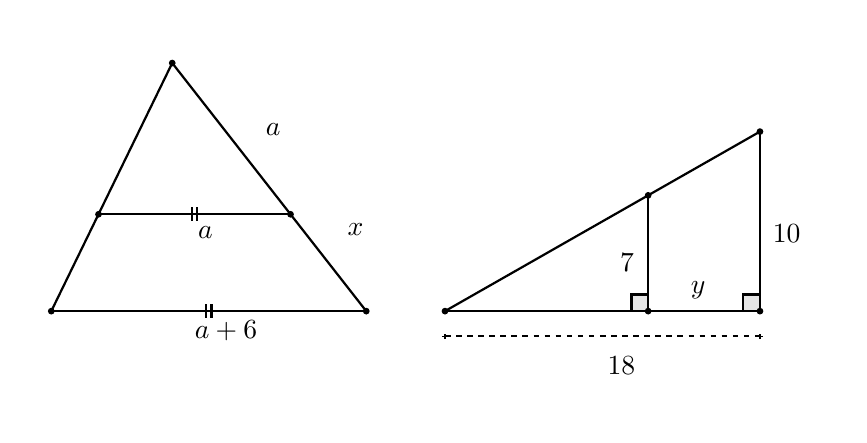
\begin{tikzpicture}
\clip(-4.3,-1.32) rectangle (6.,3.6);
\draw[line width=0.8pt,fill=black,fill opacity=0.10000000149011612] (3.58,0.21213203435596437) -- (3.367867965644036,0.2121320343559644) -- (3.367867965644036,0.) -- (3.58,0.) -- cycle;
\draw[line width=0.8pt,fill=black,fill opacity=0.10000000149011612] (5.,0.21213203435596437) -- (4.787867965644035,0.2121320343559644) -- (4.787867965644035,0.) -- (5.,0.) -- cycle;
\draw [line width=0.8pt] (-4.,0.)-- (0.,0.);
\draw [line width=0.8pt] (-2.035,0.09) -- (-2.035,-0.09);
\draw [line width=0.8pt] (-1.965,0.09) -- (-1.965,-0.09);
\draw [line width=0.8pt] (-2.4641436807847166,3.1508722475607844)-- (-4.,0.);
\draw [line width=0.8pt] (-2.4641436807847166,3.1508722475607844)-- (0.,0.);
\draw [line width=0.8pt] (1.,0.)-- (5.,0.);
\draw [line width=0.8pt] (1.,0.)-- (5.,2.28);
\draw [line width=0.8pt] (-3.4004631175077957,1.2299745105056301)-- (-0.9619031428313264,1.2299745105056301);
\draw [line width=0.8pt] (-2.216183130169561,1.3199745105056302) -- (-2.216183130169561,1.1399745105056303);
\draw [line width=0.8pt] (-2.1461831301695606,1.3199745105056302) -- (-2.1461831301695606,1.1399745105056303);
\draw [line width=0.8pt] (3.58,1.4706)-- (3.58,0.);
\draw [line width=0.8pt] (5.,2.28)-- (5.,0.);
\draw [line width=0.8pt,dash pattern=on 2pt off 2pt] (1.,-0.32)-- (5.,-0.32);
\draw (-1.4,2.5) node[anchor=north west] {$ a $};
\draw (-2.26,1.2) node[anchor=north west] {$ a $};
\draw (-0.36,1.24) node[anchor=north west] {$ x $};
\draw (-2.3,0.) node[anchor=north west] {$ a + 6$};
\draw (3.1,0.86) node[anchor=north west] {7};
\draw (5.04,1.22) node[anchor=north west] {10};
\draw (2.94,-0.46) node[anchor=north west] {18};
\draw (4,0.5) node[anchor=north west] {$ y $};
\draw [fill=black] (-4.,0.) circle (1.0pt);
\draw [fill=black] (0.,0.) circle (1.0pt);
\draw [fill=black] (-2.4641436807847166,3.1508722475607844) circle (1.0pt);
\draw [fill=black] (-3.4004631175077957,1.2299745105056301) circle (1.0pt);
\draw [fill=black] (-0.9619031428313264,1.2299745105056301) circle (1.0pt);
\draw [fill=black] (1.,0.) circle (1.0pt);
\draw [fill=black] (5.,0.) circle (1.0pt);
\draw [fill=black] (3.58,0.) circle (1.0pt);
\draw [fill=black] (5.,2.28) circle (1.0pt);
\draw [fill=black] (3.58,1.4706) circle (1.0pt);
\draw [color=black] (1.,-0.32)-- ++(-1.0pt,0 pt) -- ++(2.0pt,0 pt) ++(-1.0pt,-1.0pt) -- ++(0 pt,2.0pt);
\draw [color=black] (5.,-0.32)-- ++(-1.0pt,0 pt) -- ++(2.0pt,0 pt) ++(-1.0pt,-1.0pt) -- ++(0 pt,2.0pt);
\end{tikzpicture}\end{center}
\item {} 
Determine as medidas \(x\) e \(y\) na figura a seguir.
\begin{center}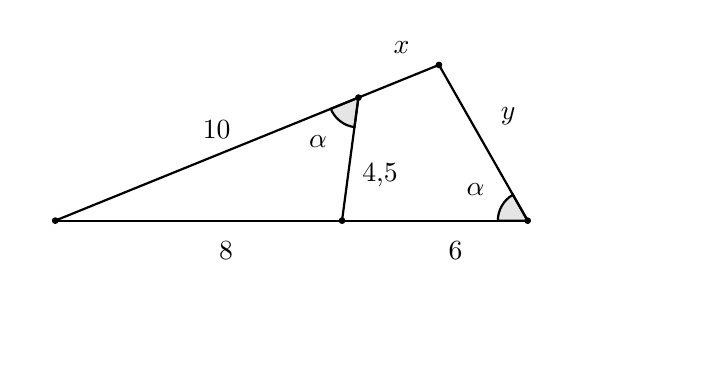
\begin{tikzpicture}
\clip(-2.3498338067109477,-1.4853536647927779) rectangle (5.844102600882048,2.450763593358133);
\draw [shift={(4.,0.)},line width=0.8pt,fill=black,fill opacity=0.10000000149011612] (0,0) -- (119.67517160754605:0.3784728132837411) arc (119.67517160754605:180.:0.3784728132837411) -- cycle;
\draw [shift={(1.8504464281507047,1.5626472567954692)},line width=0.8pt,fill=black,fill opacity=0.10000000149011612] (0,0) -- (-157.91094700933436:0.3784728132837411) arc (-157.91094700933436:-97.58611861688043:0.3784728132837411) -- cycle;
\draw [line width=0.8pt] (-2.,0.)-- (4.,0.);
\draw [line width=0.8pt] (4.,0.)-- (2.873091016604679,1.9776725767534562);
\draw [line width=0.8pt] (2.873091016604679,1.9776725767534562)-- (-2.,0.);
\draw [line width=0.8pt] (1.8504464281507047,1.5626472567954692)-- (1.6423300876403646,0.);
\draw (-0.24930969298618452,1.4) node[anchor=north west] {10};
\draw (-0.04114964568012691,-0.1417751776354958) node[anchor=north west] {8};
\draw (2.87309101660468,-0.1417751776354958) node[anchor=north west] {6};
\draw (2.1729163120297583,2.393992671365572) node[anchor=north west] {$ x $};
\draw (1.7755198580818303,0.8422541369022319) node[anchor=north west] {4,5};
\draw (3.5354184398512265,1.5613524821413407) node[anchor=north west] {$ y $};
\draw (3.1,0.6) node[anchor=north west] {$\alpha$};
\draw (1.1,1.2) node[anchor=north west] {$\alpha$};
\draw [fill=black] (-2.,0.) circle (1.0pt);
\draw [fill=black] (4.,0.) circle (1.0pt);
\draw [fill=black] (2.873091016604679,1.9776725767534562) circle (1.0pt);
\draw [fill=black] (1.8504464281507047,1.5626472567954692) circle (1.0pt);
\draw [fill=black] (1.6423300876403646,0.) circle (1.0pt);
\end{tikzpicture}\end{center}
\item {} 
Um turista em São Paulo visitou o parque do Ibirapuera e, ao sair, quis saber a que distância estava a estação do Metrô mais próxima. Consultando seu mapa, o turista identificou que encontrava-se no ponto A e que a estação Paraíso estava no ponto B, como se vê na figura a seguir.

\begin{figure}[H]
\centering

\noindent\includegraphics[width=225bp]{{FigSem-21}.png}
\end{figure}

A escala do mapa que o turista consultou era de 1/300 e, a distância AB nesse mapa era de $4{,}8$ cm.

Que distância o turista teria que caminhar até o Metrô?

\item {} 
Determine o lado do quadrado inscrito em um triângulo de base \(a\) e altura \(h\), como na figura abaixo.
\begin{center}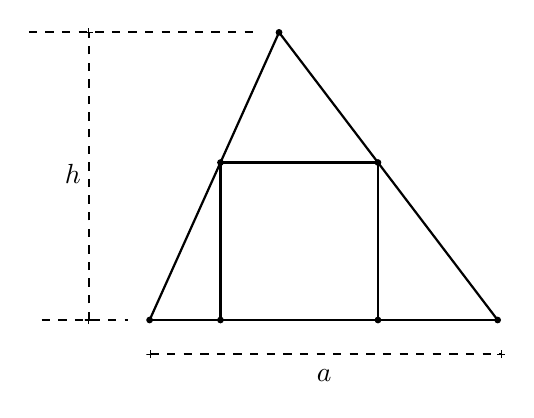
\begin{tikzpicture}
\draw [line width=0.8pt] (0.,0.)-- (0.,2.);
\draw [line width=0.8pt] (0.,2.)-- (2.,2.);
\draw [line width=0.8pt] (2.,2.)-- (2.,0.);
\draw [line width=0.8pt] (-0.9,0.)-- (3.52,0.);
\draw [line width=0.8pt] (3.52,0.)-- (0.7438016528925621,3.6528925619834713);
\draw [line width=0.8pt] (0.7438016528925621,3.6528925619834713)-- (-0.9,0.);
\draw [line width=0.8pt,dash pattern=on 3pt off 3pt] (-2.434545454545454,3.6528925619834713)-- (0.4927272727272726,3.6528925619834713);
\draw [line width=0.8pt,dash pattern=on 3pt off 3pt] (-2.270909090909091,0.)-- (-1.18,0.);
\draw [line width=0.8pt,dash pattern=on 3pt off 3pt] (-0.8890909090909092,-0.4327272727272719)-- (3.565454545454545,-0.4327272727272719);
\draw [line width=0.8pt,dash pattern=on 3pt off 3pt] (-1.670909090909091,0.)-- (-1.670909090909091,3.6528925619834713);
\draw (1.1,-0.5) node[anchor=north west] {$ a $};
\draw (-2.1,2.1) node[anchor=north west] {$ h $};
\draw [fill=black] (0.,0.) circle (1.0pt);
\draw [fill=black] (2.,0.) circle (1.0pt);
\draw [fill=black] (0.,2.) circle (1.0pt);
\draw [fill=black] (2.,2.) circle (1.0pt);
\draw [fill=black] (-0.9,0.) circle (1.0pt);
\draw [fill=black] (3.52,0.) circle (1.0pt);
\draw [fill=black] (0.7438016528925621,3.6528925619834713) circle (1.0pt);
\draw [color=black] (-0.8890909090909092,-0.4327272727272719)-- ++(-1.5pt,0 pt) -- ++(3.0pt,0 pt) ++(-1.5pt,-1.5pt) -- ++(0 pt,3.0pt);
\draw [color=black] (-1.670909090909091,0.)-- ++(-1.5pt,0 pt) -- ++(3.0pt,0 pt) ++(-1.5pt,-1.5pt) -- ++(0 pt,3.0pt);
\draw [color=black] (-1.670909090909091,3.6528925619834713)-- ++(-1.5pt,0 pt) -- ++(3.0pt,0 pt) ++(-1.5pt,-1.5pt) -- ++(0 pt,3.0pt);
\draw [color=black] (3.565454545454545,-0.4327272727272719)-- ++(-1.5pt,0 pt) -- ++(3.0pt,0 pt) ++(-1.5pt,-1.5pt) -- ++(0 pt,3.0pt);
\end{tikzpicture}\end{center}
\item {} 
Carlos e sua esposa Joana estavam visitando Buenos Aires e ao passar pelo enorme obelisco que fica na Praça da República, ele teve a curiosidade de saber sua altura.

\begin{figure}[H]
\centering

\noindent\includegraphics[width=300bp]{{FigSem-23}.png}
\end{figure}

Joana que é engenheira e tem sempre uma pequena trena na bolsa disse o seguinte: Caminhe sobre a sombra do obelisco e conte seus passos. Procure dar passos iguais. Carlos fez o que ela pediu e encontrou 44 passos para o comprimento da sombra.

Em seguida, ela pediu a Carlos que ficasse em pé e mediu a sombra de Carlos no chão, encontrando $87$ centímetros. Pediu ainda que Carlos desse um passo do tamanho que ele usou para caminhar sobre a sombra e encontrou $70$ cm para o comprimento do passo. Como Joana sabia que Carlos possui 1,80m de altura, ela pode determinar a altura do obelisco.

Com os dados dessa história, determine um valor aproximado para a altura do obelisco.

\item {} 
A figura a seguir mostra uma sequência de três triângulos equiláteros sendo que os dois primeiros possuem lados medindo 8 e 6.
\begin{center}\begin{tikzpicture}
\begin{scope}[scale=.35]
\fill[line width=0.8pt,color=\currentcolor!80,fill=\currentcolor!80,fill opacity=0.15000000596046448] (0.,0.) -- (8.,0.) -- (4.,6.9282032302755105) -- cycle;
\fill[line width=0.8pt,color=\currentcolor!80,fill=\currentcolor!80,fill opacity=0.15000000596046448] (8.,0.) -- (14.,0.) -- (11.,5.196152422706633) -- cycle;
\fill[line width=0.8pt,color=\currentcolor!80,fill=\currentcolor!80,fill opacity=0.15000000596046448] (14.,0.) -- (18.5,0.) -- (16.25,3.897114317029974) -- cycle;
\draw [line width=0.8pt,color=\currentcolor!80] (0.,0.)-- (8.,0.);
\draw [line width=0.8pt,color=\currentcolor!80] (8.,0.)-- (4.,6.9282032302755105);
\draw [line width=0.8pt,color=\currentcolor!80] (4.,6.9282032302755105)-- (0.,0.);
\draw [line width=0.8pt] (4.,6.9282032302755105)-- (32.,0.);
\draw [line width=0.8pt,color=\currentcolor!80] (8.,0.)-- (14.,0.);
\draw [line width=0.8pt,color=\currentcolor!80] (14.,0.)-- (11.,5.196152422706633);
\draw [line width=0.8pt,color=\currentcolor!80] (11.,5.196152422706633)-- (8.,0.);
\draw [line width=0.8pt,color=\currentcolor!80] (14.,0.)-- (18.5,0.);
\draw [line width=0.8pt,color=\currentcolor!80] (18.5,0.)-- (16.25,3.897114317029974);
\draw [line width=0.8pt,color=\currentcolor!80] (16.25,3.897114317029974)-- (14.,0.);
\draw [line width=0.8pt] (0.,0.)-- (32.,0.);
\draw (3.9951310905372663,-0.5041937742192144) node[anchor=north west] {8};
\draw (11.082050730853824,-0.5041937742192144) node[anchor=north west] {6};
\draw (16.248216449963092,-0.5041937742192144) node[anchor=north west] {$ x $};
\draw (-0.6411714778941265,-0.3717279865497462) node[anchor=north west] {$A$};
\draw (32.144110970299295,-0.10679641121080977) node[anchor=north west] {$B$};
\end{scope}
\end{tikzpicture}\end{center}\begin{enumerate}
\item {} 
Calcule o lado do terceiro triângulo.

\item {} 
Quanto mede o segmento AB?

\end{enumerate}

\item {} 
Seja ABCD um retângulo e \(M\) um ponto do lado \(CD\). São dadas as medidas: \(BC = 5\), \(CM = 4\) e \(MD = 2\). O ponto \(P\) é o ponto de interseção dos segmentos \(AC\) e \(MB\). Calcule as distâncias de \(P\) aos quatro lados do retângulo.

\end{enumerate}










\ifnum\aluno=1
\clearpage
\else
\notasfinais
\fi


\bibliography{../Bibliografia/probabilidade1_bibliografia.bib}

\nocite{*}
